\documentclass[11pt,letterpaper]{report}
\usepackage{listings} % Allow listing of source codes
\usepackage{tikz}
\usetikzlibrary{shapes, arrows, shadows}
\usepackage{graphicx}   % Required to use pictures
\usepackage{cite}
\usepackage{hyperref}  % \url command for bibliography entries
\usepackage{setspace}   % Control line spacing
\usepackage{etoolbox}
\apptocmd{\sloppy}{\hbadness 10000\relax}{}{}
% Suppress underfull bad box(es) for some bibliography entries
\lstset{numbers=left,
numberstyle=\tiny,basicstyle=\small,
tabsize=2,breaklines,showstringspaces=false,frame=tB}
\lstset{literate=
{ö}{{\"o}}1
{ä}{{\"a}}1
{ü}{{\"u}}1
{Ö}{{\"O}}1
{Ü}{{\"U}}1
{Ä}{{\"A}}1
{ß}{{\ss{}}}1}

\title{Structured Repository of Information Related to Software Certification}
\author{
        \normalsize
        Ishwaree Argade
            \mbox{}\\ %
        \normalsize MEng (Computer Science)
         \mbox{} \\
       \normalsize Department of Computing and Software 
                \mbox{}\\ %
        \normalsize McMaster University 
        \mbox{} \\
        \date{\today} \\
}


\begin{document}
\maketitle

\begin{abstract}

Software certification is the process of collecting evidence that the (software) parts of a software intensive system satisfies its requirements.  As this is a rather new field, it is important to collect current materials on this topic, to serve as reference material.  This is the particular task described here: choosing, indexing and classifying various materials pertaining to software certification, with an eye towards searchability and reuse.  For concreteness, rather than selecting all materials, three areas were chosen: challenge problems, course modules, and certified libraries (with their accompanying tools).  The data thus collected was made into a repository.  A choice was made to use standard technologies (XML, Schema, XSL, etc) for this purpose, to leverage the great many tools already in existence.

Throwing data into a repository is insufficient for searchability and reusability.  At the very least, the data needs to be described in a relatively uniform manner.  Thus, after an initial data gathering process was done, commonalities in the meta-data associated with each area (challenge problems, etc) were identified.  These were then codified in a Schema (using XSD), one per area.  The design of these schemas is explained, and their adequacy is verified by instantiating it with some data.  For human understandability of the results, we also created some XSL to display the data, guided by the schema.  
\end{abstract}

\setcounter{tocdepth}{2}
\tableofcontents

\chapter{Introduction}

Software Certification deals with the process of certifying a system containing some software inside it, but restricting the certification process to the software aspect only \cite{seminar}. The certification process ensures the reliability and safety of the software system to be certified listing all the information necessary for its assessment. It encompasses the wide range of formal, semi-formal and informal assurance techniques, which include even formal verification of security policies, system simulation, testing and code reviews \cite{SCMS}. Thus, the certificates can have different types and certification process follow various mechanisms.

The most popular approach for software certification is the process based certification of systems. The process through which a software system is developed is evaluated rather than evaluating the final product. As many software certifiers find the evaluation of software process easier than evaluation of the product itself, process based certification is widely used \cite{Lawford}. One reason for this is that it is not possible to test the final product entirely even with the help of a huge number of test cases. Hence, the focus is given on certain supportive evidences which would guarantee the quality of the software systems. Secondly, it is difficult to determine the metrics/attributes essential in assessing the final software product, more emphasis is given on the software process instead \cite{Lawford}. Some examples of this approach, like ISO 9000 and CMMI, certify that the proper engineering methods and processes are followed to manufacture the product \cite{Voas}.

Though process based certification is a general approach, it does not guarantee the reliability of the software as it focuses only on the process and not on the individual product. It certifies overall products and not a specific product. Thus, another approach called product based certification is put forward. A detailed analysis of this aspect of software certification is found in the paper by Wassyng, Maibaum, and Lawford \cite{Lawford}. According to them, the goal of the certification should be to ensure that the product satisfies certain characteristics by assessing some measurable attributes of the product. This approach to the software certification believes that there should be a mandated software development process, which would guarantee the quality of development process of the product, and then the product can be evaluated without consideration of the actual process followed to develop a specific product \cite{Lawford}.

Another certification method based on product based approach is proposed by Voas \cite{Voas}. According to him, by hiring a third party to issue software certification based on end users' feedback provides more unbiased and reliable software certification. Using this concept, he proposes a certification process involving automated methods to assess the behaviour of the software and to avoid the problem of miscertification \cite{Voas}.

Software development nowadays widely follows reusability of components. Reuse of components is an important factor to reduce the cost of software development. Thus, the reliability of the part to be reused has to be evaluated. One method to determine the reliability of software that builds the structural model and usage profile of software components and then evaluates it against a set of test cases is given by Wohlin and Runeson \cite{CSC} and is applicable to both part as well as system certification.

A software certification management system is used for management of certification \cite{SCMS}. It stores the information about different systems and varieties of certificates along with the entire certification history of the specific system. One of the challenges related to software certification is storing and providing the useful information. Hence, the goal of this report is to create a repository to store some material in various areas related to Software Certification.

This report focuses on three areas related to Software Certification namely Challenge Problems, Course Modules and Certified Software Libraries and Verification Tools to index some available material in the respective areas. These areas were already chosen by the principals running the Software Certification project at McMaster \cite{McCert}. The objective is to design a repository that would store relevant material for the areas related to software certification. The central structure of the repository is shown in \ref{Fig:1}. The repository has five main areas. However, the scope of this report is just first three areas shown in \ref{Fig:1}. 

\begin{figure}[ht]
\centering
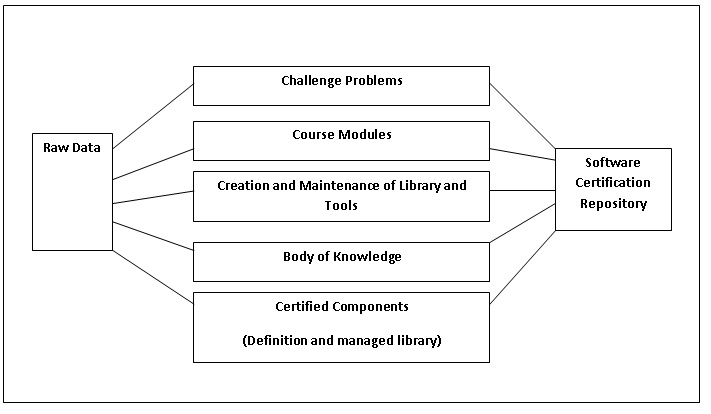
\includegraphics[width=110mm]{Images/Overview_SW_Repo.jpg}
\caption{Design of Software Repository}
\label{Fig:1}
\end{figure}
\pagebreak
The latter chapters introduce the three areas (Challenge problems, Course Modules and Certified Software Libraries)  in detail, the idea of the software repository meant to store available material around these three areas, their schema designing and testing processes, finally concluding with future scope.

\chapter{Global Requirements}
The first task here is to find the reference material in all the three areas. The next step is to provide a mechanism to store the gathered material in a uniform format. This can be accomplished be designing a schema using the meta-data for each area. The material is analyzed and various elements describing the particular area are found. The meta-data gathered can contain specific information. Hence, the next requirement would be to find the common elements in all the meta-data gathered to figure out the attributes for the schema. This then builds the foundation for schema implementation for each of the chosen areas.\newline

\noindent The requirements can be listed as follows: 
\begin{itemize}
\item \textbf{Finding reference material:- } The primary requirement is to find the reference material related to three chosen areas. For example, sample challenge problems like SAT Challenge, CADE ATP challenge etc, some sample course modules containing software certification contents, a set of certified libraries and verification tools were selected as reference problems for challenge problem, course modules, libraries and tools areas respectively. This completes the data gathering process for each area. 
\item \textbf{Analyzing reference material:- } The gathered data needs to be stored in a uniform structural format that makes it searchable and reusable. Schema design imposes a logical structure on the data. It organizes the information in a structured way, which makes it easy to search, index and visualize. Thus, a schema is required here to store the material in a uniform manner. Material around the three areas is independent of each other and is characterized by different attributes. Thus, the repository would have a schema design for each of the components of the repository. So, there would be separate schemas for challenge problems, course modules, libraries and tools. 

The schema designing process can be started by analyzing the gathered sample data material. For example, after analyzing twelve course modules in software certification areas, element set for each course module is found out. Element set is the important information that should be stored about the particular course module. This would give us twelve elements sets which can be called as meta-data for each of the twelve course modules. Similarly, this can be done for the other areas. 
\item \textbf{Finding common elements for each area:- } The meta-data can be specific to the corresponding data sample. For example, as explained above, after analyzing twelve course modules we get twelve sets of meta-datas, one for each course module. The meta-data describes each course module. So, the information can vary depending upon the course module content, their aims, materials used, assessment structure and rules. Thus, there is a need to find the commonalities in all the meta-data that would help to structure the important generic information about the course modules. For example, all the course modules have some description, module name, code, high level course content description, rules etc. This information can be stored in a structured format. 
\item \textbf{Schema Designs:- } The common information can be formulated in schema designs, which would allow users to store and index the material around the three areas. Thus, the respective schemas can be designed using the common elements for challenge problems, course modules, certified libraries and tools.     
\end{itemize} 

The corresponding schema designs are then implemented using standard technologies like Xml Schema Definitions (XSDs), Extensible Markup Language (XMLs) and Extensible Style Sheets (XSLs) \cite{XSD, olXSL, olXSD}.

\chapter{Overview of Software Repository}
 The design of the repository is provided by the principals running the Software Certification project at McMaster, as mentioned earlier. The report considers first three components of this repository namely Challenge Problems, Course Modules and Creation and Maintenance of Library and Tools. This chapter gives a brief overview of the three areas. The detail explanation of all the three areas is given in subsequent chapters.

 \section{Challenge Problems}
 The Challenge Problem part of the repository is meant to store some challenge problems in the area of software certification. Challenge problems are sets of prototypes in the software certification area. Examples of various challenge problems are SMT COMP challenge, CADE ATP challenge and Pacemaker challenge \cite{SAT,CADE,Pacemaker,SMT,SV}. Most of the challenge problems are offered every year as a part of various conferences and workshops held for software communities. For example, the CADE ATP System Competition (CASC) is held at each CADE and IJCAR conference. CASC evaluates the performance of sound, fully automatic, classical logic ATP systems. CASC evaluates the performance of sound, fully automatic, classical logic order ATP systems. 
 
 Challenge problems are offered in various areas such as boolean satisfiability (SAT solving), automation, object orientation, Satisfiability Modulo Theories etc. Some challenges are only open to academia while some are open to both industry and academia. Every challenge has a different set of rules, expected format of solution and system requirements to test the solutions. The repository needs to store these kinds of challenges. However, all the information related to challenge problems should be stored in such a way that would make challenges searchable and reusable. Hence, the goal is to design a schema that would capture all the generic information such as format of the problem, expected solution, rules for the challenge, available solutions, deadlines etc for all the challenges and store in a uniform format.
 \section{Course Modules}Course modules intend to have all the information about the courses involving topics in software certification. The course modules typically have some aims (key objectives on higher level), pre-requisites, content, assessment format and learning outcomes (point out outcomes in detail). The repository needs to store mainly this information. The rest of the details are explained in chapter 7. Relevant course modules are modules related to safety critical systems, real time systems and embedded systems. Some examples of such course modules are modules like `Foundations of System Safety Engineering', `Hazard and Risk Assessment' and `Real-Time Embedded Systems Programming' offered at York University and Ryerson University. Around twelve course modules from various universities are considered here as reference materials and then as a test data set.
 
 The information about course modules again needs to be stored in the uniform format. Hence, the separate schema for course module is needed. The schema mainly targets all the time independent information like aim of the course, learning outcomes, course outlines, materials etc. 
 \section{Certified Libraries and Tools}
  The last component manages information about libraries and verification tools. Libraries are of two types. It can either be a library that is a part of a verification tool or it can be a library that is verified by a verification tool. For example, Coq is a tool used for verification of libraries and contains number of libraries \cite{COQ}. Many libraries can be a part of a tool and can be verified by a tool. The repository mainly targets to save the information about the libraries. However, as tools are used to verify the libraries, it is useful to store the tools as well in the repository.
 
 Around eleven libraries and three tools are considered as reference material for this \cite{Alea,DFC, MCHIP, BCastleJava, BSharp,Glibc,COQ,CADP,STL,NUSMV,SMPS}. They are analyzed and attributes for the schemas are figured out. The schema for the library should be able to tag all the data related to a library such as its current versions, contents, downloading, tools used for compilation or verification, examples, references and dependencies, if any. Along with these elements, some additional elements like execution environment, functionalities, getting the tool are added to the tools' schema. However, even though the tools' and the libraries' schemas contain some common elements they have their own attributes too and needs to be stored separately. Thus, they have their own attribute listings and implementations. Libraries and tools are stored using different schemas.  

\chapter{Methodology} 
Data gathering is the first requirement here. Data samples for each area are searched on the web. Web sites for challenge problems can be found out via web sites of their associated conferences and workshops. For example, SV-Comp challenge for software verification is a part of International Conference on Tools and Algorithms for the Construction and Analysis of Systems (TACAS) \cite{TACAS}. Thus, all the information about SV-Comp challenge 2013 can be found out via web site of TACAS 2013. Course modules can be found out on various universities' sites. However, relevant course modules can be filtered out using keywords like safety critical systems, real time and embedded systems. Similarly, libraries and verification tools can be found out by using relevant keywords and looking at the contents of the libraries as well as the certification details. 

The material associated to each area is loosely bound, meaning that they have various optional elements and can be stored effectively using XMLs instead of relational databases. The key purpose of the repository is to provide a flexible, simple database that would be easy to search, query, update and maintain. Further use of this repository would be decided by the principals running the Software Certification project at McMaster \cite{McCert}. Relational databases impose tight dependencies and constraints on the data making it complex. This is not helpful here, as the data doesn't have dependencies and and also has too many optional attributes. Another approach is to collect all the documents in a simple text/excel file under different headings. However, this approach is error prone and not as efficient as XMLs. There can be mistakes while inserting/filtering and retrieving the data. Additionally, data parsing, querying and rendering is inefficient and complicated. XML databases are used to store data persistently in XML document format \cite{XMLDB}. So, similar to the rows in relational databases tables, we have XML documents. Data is stored in XML documents according to the corresponding XML schema design (XSD) \cite{XSD}. This would create a XML database. The database can be queried effectively using XML Path Language (XPath) \cite{XPath} and XML Query (XQuery)\cite{XQuery}. XSLs can be used to render the XML data files in the browser, thus allowing users to create views for the stored documents. 

At this stage, the main focus of this report is to design and implement the schemas for the three areas of the repository and use simple XSLs to display the XML data in the browser. This completes the fundamental step for the repository. However, as a future work, an effective but simple web portal can be designed as a front end to this XML repository that would allow users to insert, update, search and manipulate the XML documents in the database without displaying the underlying schema details to the end user. This would also create the scope for developing interactive web pages instead of just displaying data using static html pages.  Hence, by considering its future application, use of XML/XSD/XSL approach adds simplicity, flexibility and efficiency to this type of repository rather than creating a rigid relational database or just indexing documents in the text files.     

As explained earlier, the repository would have a schema design for each of the components of the repository. So, there would be separate schemas for challenge problems, course modules, libraries and tools. The schemas would be created as XSDs that would cover all the required parameters to store the required data for that component. Prior to the actual schema implementation, some data samples are analyzed and attributes are figured out as explained in the requirement gathering process. The schema is then implemented using the attribute listing. The corresponding XMLs are validated against the corresponding XSD schemas using an online tool \cite{olXSD}. Finally, XSLs designed according to particular schemas of the components of the repository, are used to view XMLs in the browser. An online XSL transformer tool is used to transform XML using the respective XSL into HTML code \cite{olXSL}. This HTML is then viewed in the browser. This process is repeated for all the components of the repository. 

The subsequent chapters of the report document the entire process of schema designing, XML, XSL creation and provide sample of schemas and overview of the testing process. The source code of the project is stored in a git repository at \url{https://github.com/ish1289/MEng_Project_Final}.

\chapter{Challenge Problems}

Challenge problems are sets of prototypes of problems in software certification area. The software repository intends to store all the available and relevant challenge problems including both solved and unsolved challenge problems. The solution is also saved if it is available. Challenge problems can be a part of several conferences held for the software community. For example, there are challenges called SAT challenge, CADE ATP  challenge, Pacemaker challenge, SMT COMP challenge, SV-COMP challenge \cite{SAT,CADE,Pacemaker,SMT,SV,TACAS,SATEvent,CADEConference,IJCAR}, etc. have been offered as a part of various conferences and workshops. Each challenge has different dimensions. The sample dataset for challenge problems consists of following challenges:- 
\begin{itemize}
\item \textbf{SAT Challenge:- } SAT challenge revolves around the problems in SAT solving area. The SAT Challenge is a competitive event for solvers of the Boolean Satisfiability (SAT) problem. The event organized in 2012 is considered here. It is organized as a satellite event as a part of International Conference on Theory and Applications of Satisfiability Testing in 2012. The details of this challenge can be found out at \url{http://baldur.iti.kit.edu/SAT-Challenge-2012/} \cite{SAT}
\item \textbf{The CADE ATP System Competition:- } This competition offers problems in automation deduction area. This dataset considers challenge problem offered 2013. The CADE and IJCAR conferences are the major forums for the presentation of new research in all aspects of automated deduction. To stimulate ATP research and system development, and to expose ATP systems within and beyond the ATP community, the CADE ATP System Competition (CASC) is held at each CADE and IJCAR conference. The details can be found out at \url{http://www.cs.miami.edu/~tptp/CASC/} \cite{CADE}
\item \textbf{Satisfiability Modulo Theories Competition (SMT-COMP):- } It focuses on Satisfiability Modulo Theories Solvers. The SMT workshop will include a block of time to present the competitors and results of the SMTCOMP competition. The Satisfiability Modulo Theories Competition (SMT-COMP) arose from the SMT-LIB (Satisfiability Modulo Theories Library) initiative to spur adoption of the common, community-designed SMT-LIB formats, and to spark further advances in SMT, especially for verification. The dataset considers problem offered in 2012. Details are found at \url{http://smtcomp.sourceforge.net/2012/index.shtml}. \cite{SMT}
\item \textbf{Competition on Software Verification (SV-COMP):- } This competition offered challenge problems in the area of software verification. There are several new and powerful software-verification tools around, but they are very difficult to compare. The reason is that no widely distributed benchmark suite is available and most concepts are only validated in research prototypes. This competition wants to change this. Thus, one of the goals of this competition is to establish a set of benchmarks for software verification in the community. This means to create and maintain a set of programs together with explicit properties to check, and to make those publicly available for researchers to be used in performance comparisons when evaluating a new technique. The details of the challenge considered here are found at \url{http://sv-comp.sosy-lab.org/2013/index.php} \cite{SV}
\item \textbf{Pacemaker Formal Methods Challenge:- } This is the challenge to the formal methods community hosted by Software Quality Research Laboratory (SQRL). The details are found at \url{http://sqrl.mcmaster.ca/pacemaker.htm}. \cite{Pacemaker}
\end{itemize}

The requirements and specifications depend upon the actual challenge problem and the committee who is putting forward this challenge. As the purpose of the repository is to collect all the challenge problems, a general schema which would be able to catch all the information of diverse challenge problems is needed. The schema provides a schematic structure to the repository in order to store challenge problems.  

\section{Schema Design} 
The first step in schema designing process is to analyze different challenge problems and try to find out some attributes that are common in all the challenges. The collective attributes are the various parameters in different challenges that make it possible to preserve their information in a structured manner. 

As specified earlier, the schema is designed using XSD. Thus, all the information is tracked in the form of tags using XMLs. The XMLs of various challenges are then validated against the same created schema. The schema portrays the general structure for all the challenges still allowing users to embed challenge problem specific information in the XMLs. 

Meta-data in the form of attributes is collected. The meta-data depicts the information of the particular challenge. For example, in case of SAT challenge, its organization, location, tracks allowed, its assessment, hardware/software requirements, supporting documentation, available solutions, result details, benchmark details, input/output specifications are noted down. This is done for five challenge problems mentioned above. 

The next task is to find common attributes using all the meta-datas. The common attributes eliminate all the challenge specific information, but keep the generic information such as location, supporting documentation, deadlines etc. The challenge specific information also can be stored in a generic format. For example, each challenge has different rules, assessment process and execution environment. Some challenges have benchmark problems which are sets of small challenges and they have to be solved before facing the actual challenge. However, all this challenge specific information can also be stored in a generic way. The schema provides tags to store generic information along with the tags which points to the links giving specific information about the challenges.

The attribute list starts with the challenge name. Challenge name is unique for each challenge and thus acts as a primary key. The next attribute denotes the area of the challenge (SAT Solving, Automated Deduction, Object Oriented Systems). Challenge description contains information such as description, associated conference, start and end date, series information and location. Each rule can be tagged with generic attributes like category, description, input/output requirements and links that point to specific information. All the supporting documentation is stored using document name, its description and the link to the document. All types of documents including books, online materials, tutorials and discussions can also be stored in this way. 

Every challenge has different methods for assessment. However, some generic attributes can be used to store all the assessment related information for all the challenges. Assessment description, jury contact details (name, phone, email, web page link), score details and link to specific information together describe the whole assessment information. The score details may contain different points for different levels. So, it is described using special attributes 'points' and 'description'. A challenge can be open for all people or academia or industry people. The participant tag along with the description denotes information about the participants. Some challenges have benchmarks as mentioned earlier. Each benchmark has a category, description, a specified format and a deadline. Specific information related to benchmarks is stored using links.

Every challenge problem specifies a format in which a solution should be provided. It can be an executable solution, a formal specification or some other format. So, all the allowed solution forms are stored by allowed forms attribute. Input/output requirements for challenges are different for different challenges but can be captured by generic attributes input/output requirements. Execution environment details such as compilers, processors, compatible OS, allowed libraries for the solution are captured using respective tags. The execution environment in most challenge problems describes the test environment in which the solution would be tested.  The solutions for solved challenge problems are also stored in a similar way. Various deadlines information like name, description and date is captured using separate deadline tag. Most of the challenge problems allow the use of some external tools. This information is captured under tools. Results of the challenge problem if available are tagged under results. However, the results are stored in the form a link which points to the specific results information page. Some challenge problems also have information describing the changes from previous challenge. This information is captured using the description and the link to specific information if available for each change.    

Attributes' names indicate the purpose of the attribute. Therefore, this listing of attributes provides a hierarchical structure to tag information about various challenge problems and thus makes it convenient to implement this schema design using XSD. The Listing \ref{lst:attCP} in appendix A shows all the attributes derived after analyzing some challenge problems.

\section{Implementation}
The above schema design is implemented using XSD. The schema is designed to store a wide range of challenge problems and not for some specific challenge problem. Therefore, the schema contains many optional attributes which add to the flexibility to the schema. For example, in case of contact details, any available contact such as email, phone of web page link can be stored. Additionally, the schema does not even impose the restriction on number of phones, emails or web page links and allows collecting any number of contacts. Similar constraints are imposed on all other tags such as rules, supporting documents, assessment details, benchmarks, execution environment etc. This allows users to store the  maximum amount of information using available details. For example, any number of rules can be stored even if some information is absent in the rules. One rule may contain input/output requirements while the other may only contain the description and the link. Hence, the schema is implemented in a flexible way by considering all the possibilities in a set of challenge problems. All the links are implemented using Xlink. This permits us to save the links along with the description of the link.    

The whole schema is broken down into three schemas. The first one has all the elements common to the areas covered in this report meaning that it includes all the attributes common in the areas of challenge problems, course modules, libraries and tools. The second schema contains the elements required to tag detail information regarding execution environment. The third schema is the actual main schema for challenge problem that includes the above two schemas. An online tool is used to validate XMLs against this schema \cite{olXSD}.

\subsection{Common Schema}
As described earlier, this schema represents all the common attributes to the three areas covered. This is done to avoid redundancy in implementing the entire schema. The common parts mainly contains information of common types like contacts, supporting documents, related links and tools, which is common to all the three areas. This schema would be included in all the main schemas for challenge problems, course modules, libraries and tools. The Listing \ref{lst:Pcommon} displays the pseudo code for the common schema and the listing \ref{lst:common} in appendix B shows the code of common schema. All the pseudo codes given here are written using notation similar to Clafer notation which uses regular expression notation in its types \cite{Clafer}.    

\lstinputlisting[label=lst:Pcommon,escapeinside={@}{@},caption = {Pseudo Code : Common Schema}]{Code/Pseudo_Common_Schema.txt}

\subsection{Schema for Execution Environment}
This schema represents particularly the information specific to the execution environment for the challenge problems. It separates all the execution environment data from the other elements of challenge problems such as its description, assessment details, contacts, etc. This schema stores data like expected solution format, libraries, compilers, processors and OS permissible to solve a challenge and  all the elements needed to describe the required solution as well as existing solutions. The Listing \ref{lst:PExEn} shows the pseudo code for Execution Environment Schema and the listing \ref{lst:ExEn} in appendix B gives the code for the same.

\lstinputlisting[label=lst:PExEn,escapeinside={@}{@},caption = {Pseudo Code : Execution Environment Schema}]{Code/Pseudo_Execution_Environment_Schema.txt}

\subsection{Challenge Problem Schema}
This is the main schema for challenge problems. The structure of the schema is according to the schema design described earlier. It includes the two supporting schemas viz. Common Schema and Execution Environment Schema explained in the above subsections. The Listing \ref{lst:PCPSchema} displays the main elements in challenge problem schema and the listing \ref{lst:CPSchema} shows a part of the implementation.

The entire code for schema can be found \url{https://github.com/ish1289/MEng_Project_Final/tree/master/XmlSchema_ChallengeProblems/Schema}

\lstinputlisting[label=lst:PCPSchema,escapeinside={@}{@},caption = {Pseudo Code : Challenge Problem Schema}]{Code/Pseudo_Challenge_Problems.txt}

\section{Viewing Data in Browser}
The data stored in the repository is in the form of XMLs that are validated against the above schema designed for Challenge Problems. Hence, some mechanism is needed to visualize those XMLs in the browser making them easy to interpret and read. This is done using XSLT. XSL is used to transform XML code into HTML code that is read by the browser and thus displays the contents of the XML file in the form of a html page. 

The XSL for challenge problem reads the contents from the XML files according to the challenge problem schema and displays the information in a proper format if it is present in the XML file. An online tool is used to transform XML with XSL \cite{olXSL}. The tool accepts both the XML and XSL and then transforms XML code into HTML code understood by the browser. This html file is then viewed in the browser. Thus, XSL is used to display the data stored in the repository in readable format. The entire code for challenge problem XSL is found \url{https://github.com/ish1289/MEng_Project_Final/tree/master/XmlSchema_ChallengeProblems/XSLT}.
The testing of the above schemas and XSL along with a case study is described in detail later in the report. 

\chapter{Course Modules}
The software repository collects some course modules related to software certification area \cite{York,Waterloo, MaC,Victoria}. Thus, the main objective behind this schema designing process is to identify the essential elements in several programs offered in these areas. These elements should provide a schematic structure to be able to tag all the information related to various courses. Some examples of course modules are courses related to safety critical systems, embedded systems and real time systems. Hence, relevant course modules are those, which are related to some systems containing software configuration. The sample set of course module used here contains nine course modules offered at York University, Canada, one course module offered at Victoria University, Australia and one at McMaster University, Canada. The sample dataset of course modules contains following course modules. 
\begin{itemize}
\item \textbf{Course Modules offered at York University:- } York University in Canada offers nine course modules as a part of MSc program in Safety Critical Systems. The details about each module include course contents, aims, learning outcomes, assessment details, rules of the modules etc. All this information can be found out at \url{https://www.cs.york.ac.uk/postgraduate/taught-courses/msc-scse/#tab-2}. \cite{York}   
\item \textbf{Real-Time Systems:- } This is a course module offered at McMaster University. The module mainly focuses on teaching students how to build computer systems that can be trusted in situations where the system's response to external events must be both timely and accurate. The details are found out at \url{http://www.cas.mcmaster.ca/~downd/courses/4aa4/4aaout.htm} \cite{MaC}
\item \textbf{Embedded Computer Systems:- } The course module is offered at University of Waterloo. The module provides students with the knowledge and skills to design modern embedded systems. More information is located at 
\url{https://ece.uwaterloo.ca/~rpellizz/ECE423.php} \cite{Waterloo}
\item \textbf{Embedded and Networked Systems:- } Victoria University in Australia offers this relevant course module.
It includes basic concepts of computer communication. Link to the course module is \url{http://www.vu.edu.au/units/ENE3202}.
\end{itemize}

\section{Schema Design}
Similar to challenge problem schema design, the first step here is again to analyze different course modules and figure out common elements. The elements altogether represent all the information of the course modules. Note that here the main focus is to collect all time independent data. Therefore, the major goal of an analysis of various challenges is to find out attributes such as learning outcomes, aim of the module, pre-requisites and contents rather than focussing on deadlines and timings.  

The course module is offered in some school/university. This information should be tagged followed by module name and module code. Module name and module code uniquely identify the course modules. Then, the professors' details offering the course module should be stored. This is done by tagging name, description, available contacts like emails, phone and web site. The next tags capture the status of course module (core/optional/Active etc.) and whether it is full-time or part-time. Some courses are allowed for certain numbers of tracks i.e. are eligible for students in certain programs. Supporting information like number of credits, teaching term, feedback, description, location, results is also captured using the appropriate tags. 

The major purpose in indexing such course modules is to get information about their aims, learning outcomes, topics covered in the courses, material used in the courses (books/online tutorials, links etc.). Information about the assessment is stored under different tag. All the assignments' and exam details using separate tags one for each assignment and exam under assessment tag. Some course modules use external tools. They are tagged under tools tag using appropriate sub-tags. Links are stored in most of the cases (aims/assessment details, tools etc.) to point to course specific information.     
 
This schema is also implemented using XSD. Thus, all the attributes found by analyzing various course modules are organized in a hierarchical structure making the translation to XSD easy. The Listing \ref{lst:attCM} in appendix A shows all the attributes used to implement course module schema.


\section{Implementation}
Similar to challenge problems, various course modules have different amount of information. So, the schema should be able to catch all the available information for the course modules. Naturally, the implemented schema has many optional elements. Some examples are feedback, workload, allowed tools, information about books etc. Some tags like aim, rule, book, pre-requisites etc. have no restrictions on number of elements. This allows users to record any number of elements. For example, there are many aims for a course module. Every aim is represented by "aim" tag inside outer tag "aims". Similarly, all rules, pre-requites, tools, learning outcomes, assignments and exams are recorded.    
The schema implementation follows the schema discussed in an above section. It also includes the common schema implemented given in Listing \ref{lst:common}. The pseudo code of common schema is given in listing \ref{lst:Pcommon}. This schema again covers the general structure to tag all the attributes of course modules in diverse areas while allowing saving some module specific data, as well. The schema is then tested with some sample course module XMLs by using an online XML schema validation tool \cite{olXSD}. The testing details are discussed later in the report.  The Listing \ref{lst:PCMSchema} shows the pseudo code for course module schema and the listing \ref{lst:CMSchema} shows the part of the implementation.
 
The complete code is found out at \url{https://github.com/ish1289/MEng_Project_Final/tree/master/XmlSchema_Course_Modules/Schema}

\lstinputlisting[label=lst:PCMSchema,escapeinside={@}{@},caption = {Pseudo Code : Course Module Schema}]{Code/Pseudo_Course_Modules.txt} 

\section{Viewing Data in Browser}
Similar to challenge problems XMLs, course module XMLs also need a XSL to transform XML code into HTML code. This makes it able to be viewed in the browser. The XSL is implemented according to the course module schema given above. It checks if the information is present in the XML or not and then converts it into appropriate HTML code. The HTML code displays information in an eye pleasing and organized format. An online tool is used to transform XMLs using this XSL \cite{olXSL}. As discussed earlier, the tool accepts both XML and XSL, then transforms the given XML according to the XSL finally providing an HTML code as output. The code for course module XSL is found \url{https://github.com/ish1289/MEng_Project_Final/tree/master/XmlSchema_Course_Modules/XSLT}

\bigskip

The testing of the XSL with some sample XMLs is done and is later discussed in the report. 

\chapter{Libraries and Tools}
The third component of the repository saves the data related to libraries and tools. Libraries can be a part of the tool or can be verified using a tool. There is a many to one relationship between tools and libraries. Tools used for verification are considered here. The main aim here is to look for the certified libraries. Some of the certified libraries are verified by verification tools. So, storing information about the tools along with the libraries is useful considering the future scope in the area. Thus, the repository requires schemas to store some certified software libraries as well as some verification software tools used in the area of software certification. Libraries and tools are related to each other. So, they have some attributes like versions, overview, content files, extensions, contacts and documentation in common. However, as libraries are smaller than tools and can be a part of tool, tools have some different downloading ways and execution environment details. Libraries can also have attributes like examples, references and dependency details. Thus, it is helpful to store libraries and tools using separate schemas in the repository and hence two separate schemas for libraries and tools are implemented respectively.   
The sample dataset for libraries contains following libraries. 
\begin{itemize}
\item \textbf{The GNU C Library (glibc):- } The GNU C Library is used as the C library in the GNU systems and most systems with the Linux kernel. The library defines the system calls and other basic facilities such as open, malloc, printf, exit etc. More information is at \url{https://www.gnu.org/software/libc/index.html} \cite{Glibc}
\item \textbf{Bouncy Castle libraries for cryptography:- } Bouncy Castle offers libraries for cryptography, one in java and one in C sharp. Both the libraries are certified. Detail information about the C sharp project is at \url{http://www.bouncycastle.org/index.html} \cite{BCastleJava, BSharp}
\item \textbf{Microchip Software Certified Libraries:- } Microchip’s MCUs and DSCs a set of certified software libraries and code examples. These libraries are mainly related to digital filters, DSP, encryption/decryption, maths and communication. The entire list of libraries is available at \url{http://www.microchip.com/SoftwareLib.aspx}. \cite{MCHIP} The sample dataset contains four libraries viz. 'Microchip Certified Class B Safety Software Library for 16 bit and PIC32 MCUs', 16-bit CPU Self-test Library, SMPS Control Library and PIC32 Audio Equalizer (EQ) Filter Library .
\item \textbf{OpenSSL:- } OpenSSL is full-strength general purpose cryptography library. The details of the library are at \url{http://www.openssl.org/}. \cite{SSL}
\item \textbf{Standard Template Library:- } The Standard Template Library, or STL, is a generic C++ library of container classes, algorithms, and iterators; it provides many of the basic algorithms and data structures of computer science. The link to the library is \url{https://www.sgi.com/tech/stl/stl_introduction.html}. \cite{STL}
\item \textbf{Alea: a library for reasoning on randomized algorithms in Coq:- } This library forms a basis for reasoning on randomised algorithms in the proof assistant Coq. The details of the library are found at \url{https://www.lri.fr/~paulin/ALEA/}. \cite{Alea}
\item \textbf{A Coq Library on Floating-Point Arithmetic:- } The library can be used by using Coq verification tools. More information about the library can be found out at \url{http://lipforge.ens-lyon.fr/www/pff/}. \cite{DFC}
\end{itemize}

The sample dataset for tools consists of following tools.
\begin{itemize}
\item \textbf{The Coq Proof Assistant:- } Coq is a formal proof management system. It provides a formal language to write mathematical definitions, executable algorithms and theorems together with an environment for semi-interactive development of machine-checked proofs. More information about Coq can be found out at \url{http://coq.inria.fr/}. \cite{COQ}
\item \textbf{Construction and Analysis of Distributed Processes:- } CADP ("Construction and Analysis of Distributed Processes", formerly known as "CAESAR/ALDEBARAN Development Package") is a popular toolbox for the design of asynchronous concurrent systems, such as communication protocols, distributed systems, asynchronous circuits, multiprocessor architectures, web services, etc. Detail information is found out at \url{http://cadp.inria.fr/}. \cite{CADP}
\item \textbf{NuSMV: a new symbolic model checker:- } NuSMV is a symbolic model checker developed as a joint project between: The Embedded Systems Unit in the Center for Information Technology at FBK-IRST The Model Checking group at Carnegie Mellon University , the Mechanized Reasoning Group at University of Genova The Mechanized Reasoning Group at University of Trento. It is an open architecture for model checking. Link to the tool is \url{http://nusmv.fbk.eu/}. \cite{NUSMV}
\end{itemize}
\section{Schema Design}
The design process again begins with some sample libraries and tools \cite{Alea, DFC, MCHIP, BCastleJava, BSharp,Glibc,COQ,CADP,STL,NUSMV,SMPS}. Around eleven libraries and three tools are considered as reference material for this.  They are analyzed and attributes for the schemas are figured out. The schema for the library should be able to tag all the data related to a library such as its current versions, contents, downloading, tools used for compilation or verification, examples, references and dependencies if any. Along with these elements, some additional elements like execution environment, functionalities, getting the tool are added to the tools' schema. However, even though the tools' and the libraries' schemas contain some common elements they have their own attributes too and needs to be stored separately. Thus, they have their own attribute listings and implementations.
\subsection{Attributes Listing: Libraries}
The analysis of some libraries such as Microchip certified libraries, COQ libraries, a PRL math library, glibc, Bouncy Castle library for Java and C sharp, SSL, and STL. The attribute listing starts with library name which is a mandatory attribute followed by optional attribute overview. The high level overview is tagged using overview description attribute and link is used to navigate to detail information page of the library. All the available versions including current and previous are stored using tags version name, description and link to the version. Attribute status is used to indicate whether it's a current or previous version. Content files in the library are stored using name, description and link tags for each content file. Dependency details, examples, references, documentation and experimental library contents are captured in similar ways. This type of name, description hierarchy allows users to tag available information in a flexible way. Any number of links can be stored using link tags. Contributors are stored using the same way used in Challenge problems and Course modules. Information on how to download the library is captured using the tags description, size and links and compatible OS. The Listing \ref{lst:attL} in appendix A shows the elements for the libraries' schema.

\subsection{Attributes Listing: Tools}
After analyzing some tools like COQ, CADP, NuSMv \cite{COQ,CADP,NUSMV}. Tools and attributes have some attributes in common. Content files, version details, name, documentation, related links, extensions, contacts, related tools and features are captured using the similar way. All the generic information is stored using mainly name and description tags and detail information is tagged using links. The major difference between the tools' and libraries' schema is the download methods and execution environment. Execution environment contains the languages used in the tool, input requirements, compatible OS, compiler and processor requirements. OS, compiler and processor requirements are stored using appropriate attributes like name, memory, version and description for each compiler, OS or processor. There can be three downloading formats for tools. Either it can be downloaded as source code or a binary file or in some other format. For source code only size, description and link is needed. However, for binary files compatible OS is also stored. Sometimes, there are some other ways to download the tools. This information is caught using description and links. The Listing \ref{lst:attT} in appendix A shows the elements for the tools' schema.
 
\section{Implementation}
As mentioned earlier, libraries and tools are related to each other. So, naturally they share some common elements which can be implemented separately. Moreover, both of these schemas also include the common schema discussed earlier in Listing \ref{lst:Pcommon}. Similar to challenge problems and course modules, these schemas also contain the optional attributes. This allows the user to store only available information and adds flexibility. Adding no restrictions on the number of elements permits the schema to store multiple elements like compilers, processors, versions, documentation, content files etc. The latter chapter talks about the testing of these schemas in detail. 
\subsection{Common Schema for Libraries and Tools}
The schema mainly includes implementation of a few common elements such as version details, contents' details and extensions. The Listing \ref{lst:PCSLT} shows the pseudo code for common schema for libraries and tools and the listing in appendix B \ref{lst:CSLT} gives the implementation for the same.
\lstinputlisting[label=lst:PCSLT,escapeinside={@}{@},caption = {Pseudo Code : Common Schema for Libraries and Tools}]{Code/Pseudo_Common_Lib_tools.txt}  
\subsection{Schema for Libraries}
The Listing \ref{lst:PSL} contains the pseudo code for libraries' schema and the listing \ref{lst:SL}
contains its implementation. 
\lstinputlisting[label=lst:PSL,escapeinside={@}{@},caption = {Pseudo Code : Schema for Libraries}]{Code/Pseudo_Libraries.txt}
\subsection{Schema for Tools}
The Listing \ref{lst:PTL} gives the implementation for tools' schema and the listing \ref{lst:TL}
shows its implementation.  
\lstinputlisting[label=lst:PTL,escapeinside={@}{@},caption = {Pseudo Code : Schema for Tools}]{Code/Pseudo_Tools.txt}

\bigskip
The complete code for libraries' and tools' schema can be found out \url{https://github.com/ish1289/MEng_Project_Final/tree/master/XmlSchema_Libraries_Tools/Schema}
\section*{View Data in Browser}
Similar to challenge problems and course modules, libraries and tools XMLs are viewed in the browser with the help of XSLs. 

XSLs for both libraries and tools are located at 
\url{https://github.com/ish1289/MEng_Project_Final/tree/master/XmlSchema_Libraries_Tools/XSLT}


\chapter{Testing}

The testing begins with preparing some sample XMLs for all the areas discussed. The whole schema design, implementation, XSLs implementation and testing process follow an iterative approach. The entire three areas viz. challenge problem, course modules and libraries and tools are tested individually. However, they follow the same testing process. 
 
\section{Test Cases}
After the schema design and implementation, an XML is prepared from a sample challenge problem, course module, library and a tool. This XML is validated against the first version of the schema. Some test cases described in the table \ref{table:test} are tested to check the strength, validity and effectiveness of the schema. According to the results, improvements are made to the schema. This process is repeated till the schema is tested against reasonable number of samples and passes all the test cases correctly without the further need of modification to an existing schema. 

The set of XML samples is then transformed using the XSL designed according to the finally tested schema. The HTML file produced as an output is tested against some test cases given in table \ref{table:test}. This again follows the iterative approach till all the test cases are satisfied.

The table \ref{table:test} lists down the test cases used for both XSDs and XSLs of challenge problems, course modules, libraries and tools.
%\thispagestyle{empty}
%\vspace*{-\baselineskip}
\begin{table}
\begin{tabular}{| l | p{2cm} | p{5cm} | p{2cm} | p{1cm} |}
\hline \textbf{Sr.No.} & \textbf{Test Case Name} & \textbf{Description} & \textbf{Applicable For} & \textbf{Result} \\ \hline 1. & Information coverage & check whether all the information is covered & XSD/XSL & Passed \\ 
\hline 2. & Appropriate attribute tagging & All the information should be tagged appropriately.  & XSD & Passed  \\  
\hline 3.& Allowance of specific information  & Specific but important information for the challenge should also be included without affecting the general structure of the schema & XSD & Passed \\ 
\hline 4.& Flexibility & Not all the elements are present in all the samples. The schema should allow users to insert only available information. Checking the use of optional attributes. & XSD/XSL & Passed. \\ 
\hline 5. & Attribute coverage & Testing on reasonable number of samples to verify all the attributes in the schema or XSL are utilized & XSD/XSL & Passed \\  
\hline 6. & Common schema & Use of common schema to implement common elements & XSD & Passed \\  
\hline 7. & Look and feel for XSL & Checking whether all the information when viewed in the browser is properly aligned and look and feel of HTML page & XSL & Passed \\ 
\hline
\end{tabular}
\caption[Table caption text]{Test Cases}
\label{table:test}
\end{table}
\pagebreak
These test cases are applicable to all the schemas and all the scenarios. However, the use of test cases can be illustrated with the help of a small example. The first design of the challenge problem schema captured all the rules using just the rule tag unlimited times. so, the XML file would contain the structure $<rules><rule></rule><rule></rule></rules>$. On the very first sample challenge, it worked fine for all the test cases. The schema provided mainly flexibility, information coverage. However, later while testing it on some other challenge, where rules had a lot of specific information, test cases failed. For example, the first test case "information coverage" failed because, the detailed information about the rule was not stored by the schema. The schema could store only the high level description of the rules. The second and third test cases failed because the schema had to store all the information only as a description. So, there was no other way to insert information about the input/output requirements or rule background or to store links. This was naturally hampering the flexibility of the schema though it was allowing multiple rules. Thus, the fourth test case also failed.

The above problem was fixed by changing the structure of the rule tag. More tags were added under the rule tag. This permitted the users to insert bigger rules' information in more categorized manner. Rule category was added to indicate the purpose of the rule. Rule description would store the main information about the rule. Some rules may contain input/out requirements. Appropriate tags and inner tags were added to catch this information. Rule information that is challenge specific is considered as detailed information. Links tag is added using XLink to store the links. Any number of links can be stored for a rule. Any of these inner tags category, links, input/output requirements are kept optional. So, if the rule is simple, only its description can be stored. If the rule contains only description and the link or the number of links, this can be caught as well. This new schema with new rule structure is again tested against the test cases using old and new sample challenge problems. All the test cases were passed as the schema covers all the information. It covers all the information, tags information properly, stores specific information and provides flexibility. In this way, the testing is carried out for all the elements in the schemas until all the test cases are satisfied on all the sample data sets. Fig \ref{Fig:2} shows this sample transformation.    
\begin{figure}[ht]
\centering
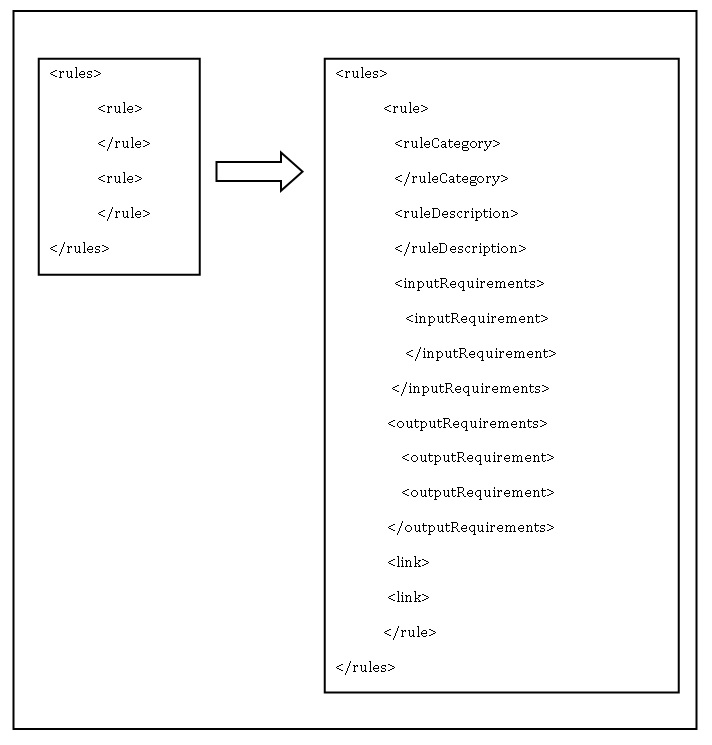
\includegraphics[width=110mm]{Images/rules.jpg}
\caption{Testing Example: Change in `Challenge Problems ``rules'' structure'}
\label{Fig:2}
\end{figure}
\section{Case Study}
This section provides a sample XML and its transformed HTML code for a challenge problem. The XMLs illustrate how the actual information is stored in the repository using the newly designed schemas and HTML files depict how the XMLs are transformed and seen in the browser using the newly implemented XSLs according to the corresponding schemas. 

Note that the report just provides one sample XML and HTML for a challenge problem. However, the schemas and XSLs are tested against five XMLs to verify their validity and effectiveness and similarly XMLs and HTMLs can be obtained for other categories and data samples. The whole set of XMLs and HTMLs for all the categories is stored in a git repository and can be viewed at \url{https://github.com/ish1289/MEng_Project_Final}

The \url{https://github.com/ish1289/MEng_Project_Final/blob/master/XmlSchema_ChallengeProblems/Sample_Xmls/XML_Challenge_Problem_SAT_Challenge.xml} gives XML for SAT challenge. The XML is prepared by extracting the information from SAT challenge website and then tagging it according to the challenge problem schema given in the Listing \ref{lst:CPSchema} \cite{SAT}. The XML is then validated using the online tool against the challenge problem schema \cite{olXSD}. The corresponding HTML can be found out at \newline \url{https://github.com/ish1289/MEng_Project_Final/blob/master/XmlSchema_ChallengeProblems/Sample_HTMLs/HTML_SAT.html}.

\chapter{Conclusion}
Software certification refers to the process of certification of the software part in the system. The report talked about some approaches to accomplish this. Component reusability is now getting popular in software certification. However, the component to be reused needs to have the appropriate certification and certification management system. One of the challenges in this area is the management of useful information regarding the certification. Therefore, the design of the software repository, which would manage information related to various areas around software certification, mainly focusing on the three areas of challenge problems, course modules and libraries and tools is proposed here.  

Future tasks for the repository can be categorized into two streams. First, would be to find more samples for all the three components discussed here. A major challenge for the work presented in the report was data gathering. It is a challenging task to find the relevant data samples. This is true for all the three areas. The second, is to create and implement schema for the rest of the two areas of the repository. The schemas can be designed and implemented by following the same methods illustrated in the report. This would complete the implementation of the proposed repository. Additional future work after the implementation of the entire repository would be a simple front end as explained in chapter 4, that would manage data queries, updates, insertions and maintenance of XML documents in the repository efficiently. Again, the use of this repository would be decided by the principals working on Software Certification project at McMaster.  

The report provides an effective mechanism to index some available material for the three areas around software certification using standard technologies such as XML, XSD and XSL.

\appendix
\chapter{Attribute Listings}
\lstinputlisting[label=lst:attCP,escapeinside={@}{@},caption = {Attributes for Challenge Problem Schema}]{Code/AttributeListingChallengeProblem.txt}

\lstinputlisting[label=lst:attCM,escapeinside={@}{@},caption = {Attributes for Course Modules Schema}]{Code/AttributeListingCourseModule.txt} 

\lstinputlisting[label=lst:attL,escapeinside={@}{@},caption = {Attributes for Libraries' Schema}]{Code/AttributeListingLibraries.txt} 

\lstinputlisting[label=lst:attT,escapeinside={@}{@},caption = {Attributes for Tools' Schema}]{Code/AttributeListingTools.txt}  

\chapter{Schema Implementations}
\lstinputlisting[label=lst:common,escapeinside={@}{@},caption = {Common Schema}]{Code/CommonSchema.txt}

\lstinputlisting[label=lst:ExEn,escapeinside={@}{@},caption = {Execution Environment Schema}]{Code/ExecutionEnvironmentSchema.txt}

\lstinputlisting[label=lst:CPSchema,escapeinside={@}{@},caption = {Challenge Problem Schema}]{Code/ChallengeProblemSchema.txt}

\lstinputlisting[label=lst:CSLT,escapeinside={@}{@},caption = {Common Schema for Libraries and Tools}]{Code/CommonSchemaLibrariesTools.txt}  

\lstinputlisting[label=lst:CMSchema,escapeinside={@}{@},caption = {Course Module Schema}]{Code/CourseModuleSchema.txt} 

\lstinputlisting[label=lst:SL,escapeinside={@}{@},caption = {Schema for Libraries}]{Code/LibrariesSchema.txt}

\lstinputlisting[label=lst:TL,escapeinside={@}{@},caption = {Schema for Tools}]{Code/ToolsSchema.txt}

\bibliographystyle{alpha}
\bibliography{References_Report_Ishwaree_Argade}

\end{document}